\documentclass[aspectratio=169,11pt,hyperref={colorlinks=true}]{beamer}
% https://github.com/zr-tex8r/BXcjkjatype/blob/master/README-ja.md
\usepackage[whole]{bxcjkjatype}
\usetheme{boxes}
\setbeamertemplate{navigation symbols}{}
\definecolor{suse}{RGB}{2, 211, 95}
\definecolor{susedark}{RGB}{13, 44, 64}
\setbeamercolor{titlelike}{fg=suse}
\setbeamercolor{structure}{fg=suse}
\hypersetup{colorlinks,urlcolor=suse}
\setbeamertemplate{footline}[frame number]
% Inserting graphics
\usepackage{graphicx}
% Side-by-side figures, etc
\usepackage{subfigure}
% Code snippits
\usepackage{listings}
% Color stuff
\usepackage{color}
% underline
\usepackage{soul}

\usepackage{amsmath}
\usepackage{tikz}
\newcommand\RBox[1]{%
  \tikz\node[draw,rounded corners,align=center,] {#1};%
}
\usepackage{hyperref}
%\usecolortheme{buzz}
%\usecolortheme{wolverine}
%\usetheme{Boadilla}
\usepackage[T1]{fontenc}
%\usepackage{fontspec}
%\usepackage[expert, deluxe]{otf}

\definecolor{mygreen}{rgb}{0,0.6,0}
\definecolor{mygray}{rgb}{0.5,0.5,0.5}
\definecolor{mymauve}{rgb}{0.58,0,0.82}


%\usepackage{CJK}
%\pdfmapline{=genshingothic@Unicode@ <genshingothic.ttf}
% bxcjkjatype
%\setgothicfont[<ID>]{<フォントファイル名>}
%\setgothicfont{/Users/foo/Library/Fonts/genshingothic.ttf}
%\setgothicfont{/Users/foo/Library/Fonts/NotoSansCJKjp-Regular.otf}
%\setgothicfont{/Users/foo/Downloads/genshingothic-20150607/GenShinGothic-P-Normal.ttf}
%\setgothicfont{/Users/foo/Downloads/genshingothic-20150607/GenShinGothic-Regular.ttf}
%\setgothicfont{hiragino.ttc}
\setgothicfont{mplus-1p-regular.ttf}
\setCJKfamilydefault{\gtdefault}
%\setCJKfamilydefault{\mcdefault}
%\CJKforce{abcdefghijklmnopqrstuvwxyzABCDEFGHIJKLMNOPQRSTUVWXYZ}


\lstset{%
  backgroundcolor=\color{susedark},   % choose the background color; you must add \usepackage{color} or \usepackage{xcolor}
  breakatwhitespace=false,         % sets if automatic breaks should only happen at whitespace
  breaklines=true,                 % sets automatic line breaking
  captionpos=b,                    % sets the caption-position to bottom
  commentstyle=\color{suse},  % comment style
  extendedchars=true,              % lets you use non-ASCII characters; for 8-bits encodings only, does not work with UTF-8
  keepspaces=true,                 % keeps spaces in text, useful for keeping indentation of code (possibly needs columns=flexible)
  keywordstyle=\color{blue},       % keyword style
%  otherkeywords={*,...},           % if you want to add more keywords to the set
  numbersep=5pt,                   % how far the line-numbers are from the code
  numberstyle=\tiny\color{mygray}, % the style that is used for the line-numbers
  rulecolor=\color{white},         % if not set, the frame-color may be changed on line-breaks within not-black text (e.g. comments (green here))
  showspaces=false,                % show spaces everywhere adding particular underscores; it overrides 'showstringspaces'
  showstringspaces=false,          % underline spaces within strings only
  showtabs=false,                  % show tabs within strings adding particular underscores
  stringstyle=\color{suse},   % string literal style
}

\setbeamerfont{caption}{series=\normalfont,size=\fontsize{6}{8}}
%\setbeamerfont{caption}{series=\normalfont,size=\large}
\setbeamertemplate{caption}{\raggedright\insertcaption\par}

\setlength{\abovecaptionskip}{0pt}
\setlength{\floatsep}{0pt}

\author[Masayuki Igawa]{%
  \texorpdfstring{%
    \centering
    Masayuki Igawa\\
    \href{mailto:masayuki@igawa.io}{masayuki@igawa.io}\\
    \texttt{masayukig on \href{http://freenode.net/}{Freenode},
     \href{https://twitter.com/masayukig}{Twitter},
     \href{https://github.com/masayukig}{GitHub}}
  }
  {Masayuki Igawa}
}
\date{11 July, 2017}
\def\place#1{\def\@place{#1}}
\place{\href{https://ospn.connpass.com/event/60330/}{@デブナイト Vol.3}}

\title[How to select good gadgets and services for diet
\hspace{2em}\insertframenumber/\inserttotalframenumber]{やせるガジェット・サービス選び方}

\setbeamercolor{background canvas}{bg=susedark}
\setbeamercolor{titlelike}{fg=white}
\setbeamercolor{structure}{fg=white}
\setbeamercolor{normal text}{fg=white}
\begin{document}

{%
% \setbeamertemplate{background canvas}{\includegraphics[width=\paperwidth,height=\paperheight]{background_title.png}}
\setbeamertemplate{footline}{}
\setbeamercolor{background canvas}{bg=susedark}
\begin{frame}[noframenumbering]
  \hypersetup{colorlinks,urlcolor=suse}
  \setbeamercolor{author}{fg=white}
  \setbeamercolor{date}{fg=white}
  \setbeamercolor{place}{fg=white}
  \titlepage{}
  \centering
  \@place \par
  \href{https://github.com/masayukig/debu-night-vol3}{github.com/masayukig/debu-night-vol3}
\end{frame}
}

% \section{Agenda}
% \begin{frame}
%   \frametitle{Agenda}
%   \begin{itemize}
%     \item 自己紹介
%     \item 自己紹介2(自分の状況)
%     \item 使ってみたガジェット・サービス
%       \item Withings, Garmin,
%       \item Runtastic(): https://www.runtastic.com/ja/results
%       \item Strava
%       \item 
%     \item おすすめすること:ガジェットは、それ単体で完結するものが良
%     い。特に、スマホ・アプリはまだまだ発展途上で動作が不安定なことが
%     多い。せっかく測定したデータがなくなったら悲しい。
%     例:体重計単体でサービス動作する。(スマホがなくても動作する。)
%     \item どうなった?(困ったこと)
%     \item まとめ
%   \end{itemize}
% \end{frame}

\section{Introduction}
\begin{frame}
  \frametitle{Disclaimer}
  \begin{itemize}
    \item 本資料は、個人の見解です。
    \item 所属する企業・団体を代表する意見ではありません。
    \item 効果・効能を保証するものでもありません。
  \end{itemize}
\end{frame}

\begin{frame}
  \frametitle{Who am I?}
  \begin{itemize}
    \item Company:SUSE/ノベル株式会社
      \begin{itemize}
        \item QE(Quality Engineering) Team
        \item[] (日本にいるのは私だけ)
        \item \href{https://www.suse.com/newsroom/post/2016/suse-acquires-openstack-iaas-and-cloud-foundry-paas-talent-and-technology-assets-from-hpe-to-accelerate-growth-and-entry-into-new-markets/}{SUSE Acquires OpenStack IaaS and Cloud Foundry PaaS Talent and Technology Assets from HPE to Accelerate Growth and Entry into New Markets}
      \end{itemize}
    \item Job: Senior Software Engineer/Open Source Programmer
      \begin{itemize}
        \item \href{https://www.openstack.org/}{OpenStack}
         \href{https://wiki.openstack.org/wiki/QA}{QA} Upstream development, Core Reviewer
        \item[] (\href{https://docs.openstack.org/developer/tempest/}{Tempest},
         \href{http://status.openstack.org/openstack-health/}{OpenStack-Health},
         \href{https://docs.openstack.org/developer/subunit2sql/}{Subunit2SQL},
         \href{https://docs.openstack.org/developer/stackviz/}{Stackviz})
        \item \href{https://www.openstack.org/}{OpenStack}
        \item \href{http://stackalytics.com/?user_id=igawa&release=all&metric=all}{stackalytics.com/?user\_id=igawa}
      \end{itemize}
    \item 2型糖尿病、BMI:26前後
  \end{itemize}
\end{frame}

\begin{frame}
  \frametitle{で?}
  \begin{center}
    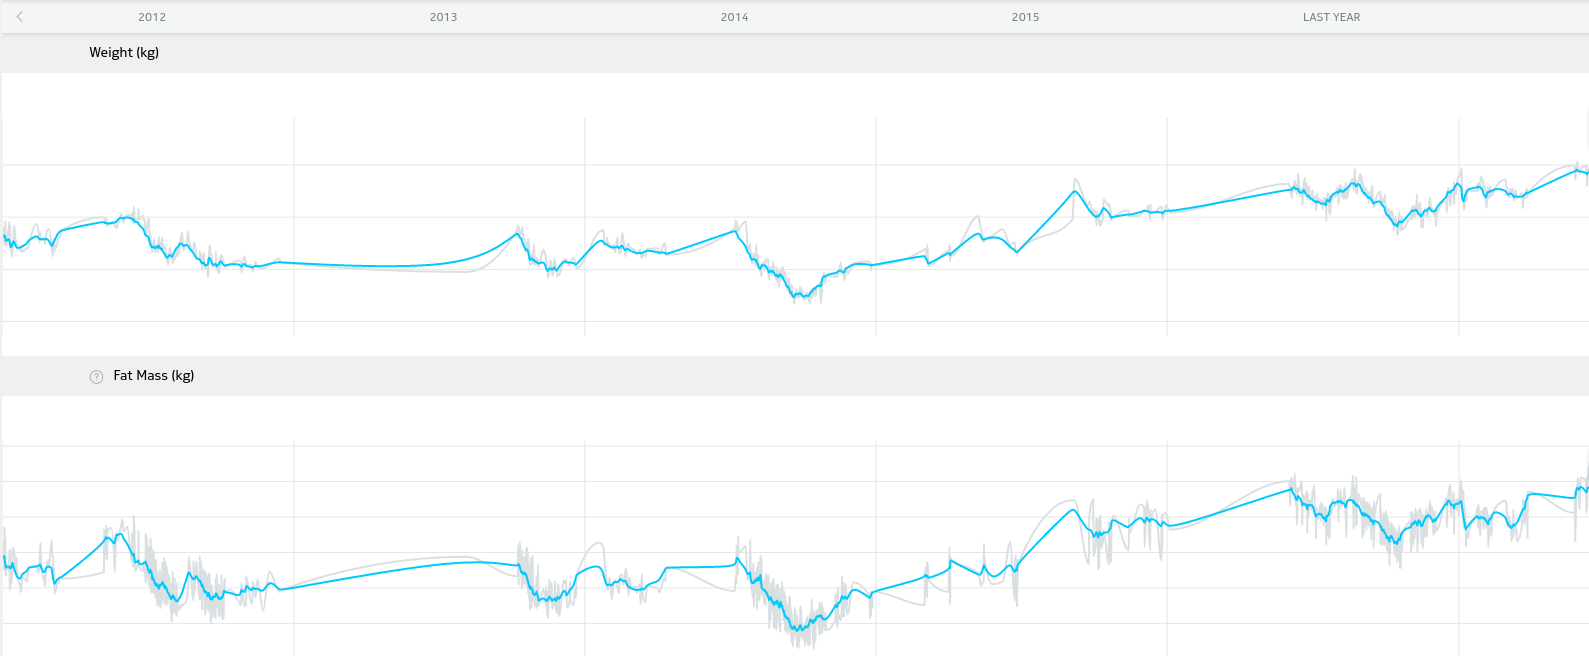
\includegraphics[width=1.0\textwidth]{my_weight.png}
  \end{center}
\end{frame}

\subsection{Main}
\begin{frame}
  \frametitle{}
  \Huge{ま、そんなにうまくいってませんw}
\end{frame}

\begin{frame}
  \frametitle{でも、うまく行ってるところもあります}
  \begin{center}
    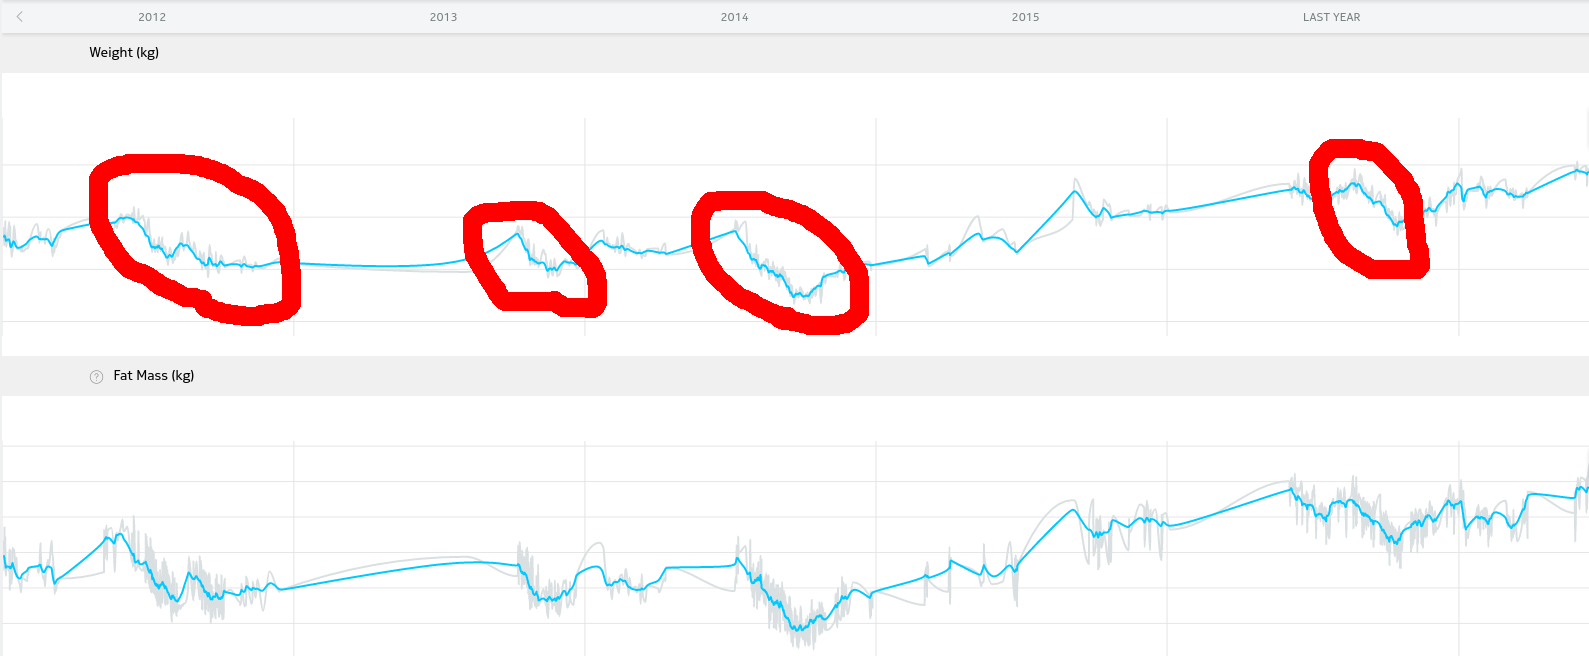
\includegraphics[width=1.0\textwidth]{my_weight_2.png}
  \end{center}
\end{frame}

\begin{frame}
  \frametitle{気に入ってるガジェット、サービスを独断と偏見で紹介します}
  なお、手っ取り早く痩せたければ、お金を払ってパーソナルトレーナー付き
  のダイエットコースの契約をしたほうが早いと思いますw
\end{frame}

\begin{frame}
  \frametitle{Withings(Nokia Health)}
  \begin{columns}[T]
    \begin{column}{.50\textwidth}
      \begin{itemize}
      \item[] 特徴
        \begin{itemize}
        \item スタイリッシュなデバイスとサービス。ヘルスケアサービスの草分
          け的存在。
        \item 最近、Nokiaに買収された。
        \end{itemize}
      \item[] Devices
        \begin{itemize}
        \item Body Cardio
        \item BPM(Blood Pressure Monitor)
        \item HR monitor
        \end{itemize}
      \item[] お気に入りポイント
        \begin{itemize}
        \item かっこいい
        \item スマホ不要のインターネット連携体重計
        \item \href{https://ifttt.com}{IFTTT.com}との連携も可能
        \end{itemize}
      \end{itemize}
    \end{column}
    \begin{column}{.50\textwidth}
      \begin{center}
        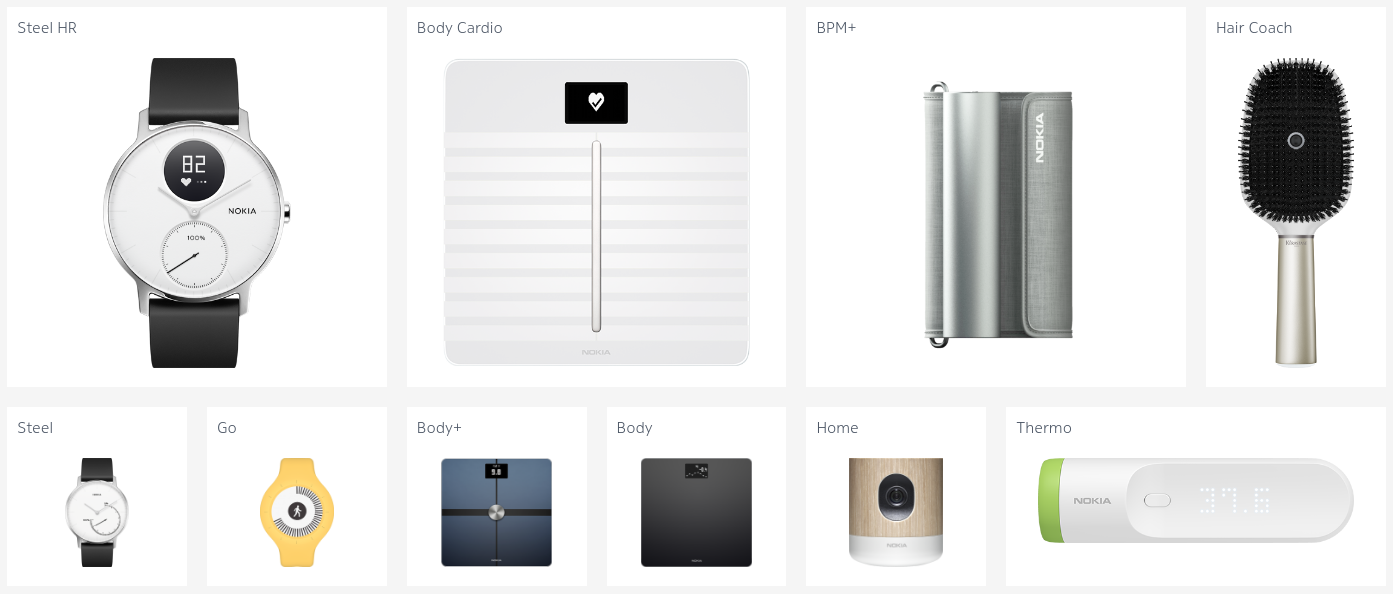
\includegraphics[width=1.1\textwidth]{withings_products.png}
      \end{center}
    \end{column}
  \end{columns}
\end{frame}

\begin{frame}
  \frametitle{Garmin}
  \begin{columns}[T]
    \begin{column}{.50\textwidth}
      \begin{itemize}
      \item[] 特徴
        \begin{itemize}
          \item GPSトラッカーの老舗。
          \item 独自仕様が多い。
          \item デバイスの値段が少し高め。
        \end{itemize}
      \item[] Devices
        \begin{itemize}
          \item HR
          \item Cycle computer + Sensors
          \item HR monitor
        \end{itemize}
      \item[] お気に入りポイント
        \begin{itemize}
          \item デバイス単体で完結
          \item スマートウォッチの電池寿命が長い(1週間くらい平気)
        \end{itemize}
      \end{itemize}
    \end{column}
    \begin{column}{.50\textwidth}
      \begin{center}
        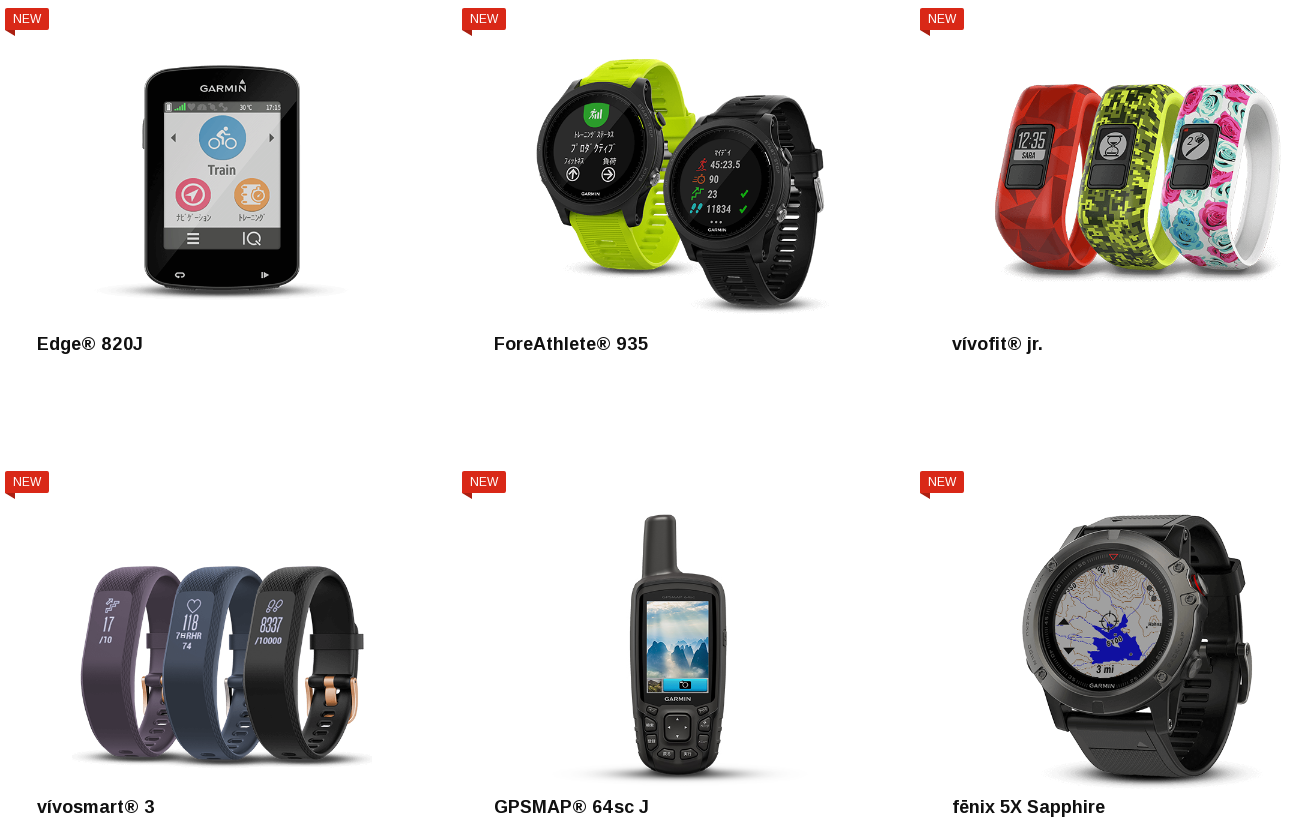
\includegraphics[width=1.1\textwidth]{garmin_products.png}
      \end{center}
    \end{column}
  \end{columns}
\end{frame}

\begin{frame}
  \frametitle{Runtastic}
  \begin{columns}[T]
    \begin{column}{.50\textwidth}
      \begin{itemize}
      \item[] 特徴
        \begin{itemize}
        \item スマホアプリ上位にランク
        \item 本格的に使おうとすると有料となることが多い
        \end{itemize}
      \item[] Devices
        \begin{itemize}
        \item 体重計
        \item アクティビティトラッカー
        \item 心拍計
        \end{itemize}
      \item[] Services
        \begin{itemize}
        \item \href{https://www.runtastic.com/ja/results}{Runtastic Results}: 結果にコミットするサービスw
        \end{itemize}
      \item[] お気に入りポイント
        \begin{itemize}
        \item \href{https://www.runtastic.com/ja/results}{Runtastic
          Results}は、ギリギリきついトレーニングメニューを出してくるの
          で、ちゃんとやると効果を実感できます。
        \end{itemize}
      \end{itemize}
    \end{column}
    \begin{column}{.50\textwidth}
      \begin{center}
        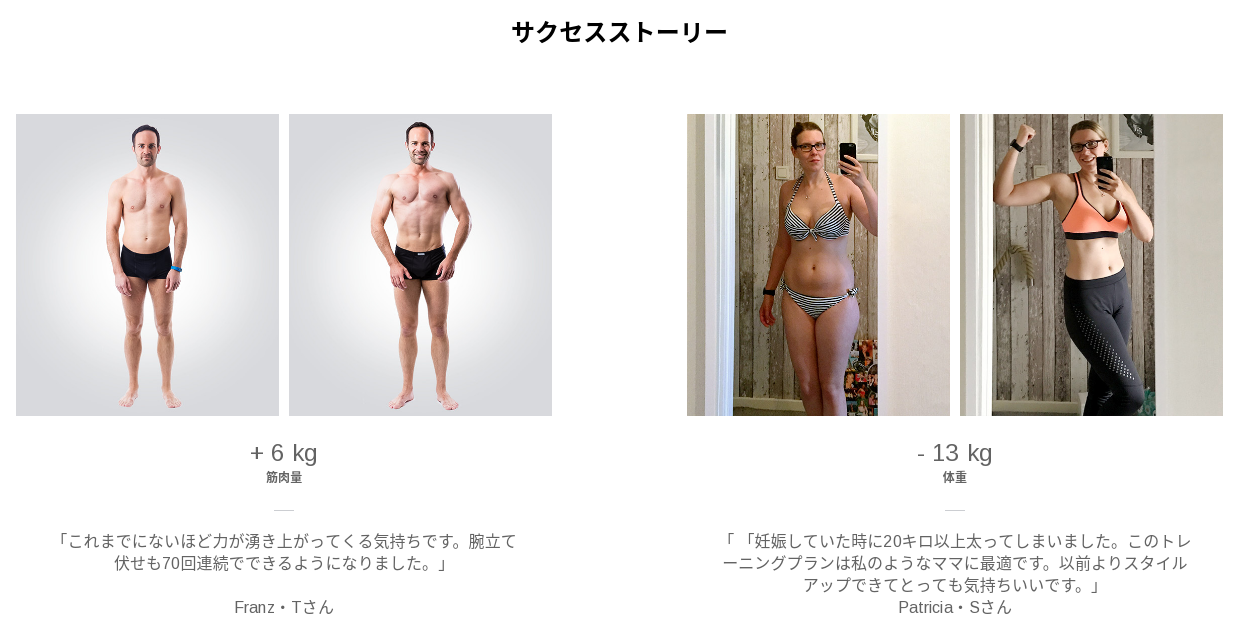
\includegraphics[width=1.1\textwidth]{runtastic_results.png}
      \end{center}
    \end{column}
  \end{columns}
\end{frame}

\begin{frame}
  \frametitle{Strava}
  \begin{columns}[T]
    \begin{column}{.50\textwidth}
      \begin{itemize}
      \item[] 特徴
        \begin{itemize}
        \item スポーツでつながるSNS
        \item 自分との勝負にも使える
        \item バーチャルに他の人と競い合える
        \end{itemize}
      \item[] お気に入りポイント
        \begin{itemize}
        \item 自動的にログが溜まっていく
        \item 自分の成長が確認できる
        \end{itemize}
      \end{itemize}
    \end{column}
    \begin{column}{.50\textwidth}
      \begin{center}
        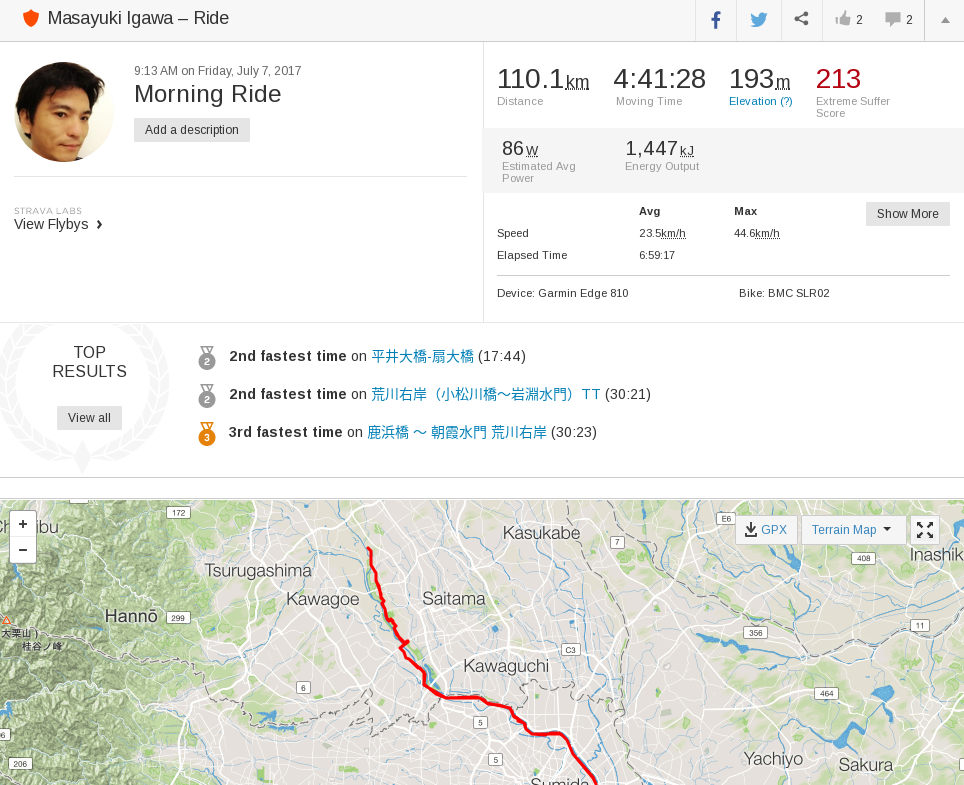
\includegraphics[width=1.1\textwidth]{strava_1.png}
      \end{center}
    \end{column}
  \end{columns}
\end{frame}

\begin{frame}
  \frametitle{その他}
  \begin{itemize}
    \item \href{https://www.google.com/fit/}{Google Fit}
    \item \href{https://www.apple.com/lae/ios/health/}{Apple Health}
    \item \href{http://30dayfitnesschallenge.co.uk/}{30 Day Fitness Challenge}
  \end{itemize}
\end{frame}

\subsection{Conclusion}
\begin{frame}
\frametitle{Conclusion}
  \begin{itemize}
  \item[] おすすめすること
    \begin{itemize}
    \item ガジェットは、それ単体で完結するものを選ぼう
    \item[] スマホ・アプリはまだまだ発展途上で動作が不安定なことが多い。
    \item[] → せっかく測定したデータがなくなったら悲しい。
    \item[例] 体重計
    \item 一人でやるのはつらい。→ 競争・励まし合う仲間を作ろう!
    \item[例] 配偶者、兄弟・姉妹、友人、SNS, マンツーマンコーチ、 etc.
    \end{itemize}
  \end{itemize}
  \begin{itemize}
  \item[] 困ったこと
    \begin{itemize}
      \item 痩せるのはできるけど、維持が難しい。
      \item 最近、痩せにくくなってきた気がする。。
    \end{itemize}
  \end{itemize}
\end{frame}

\subsection{More Information}
\begin{frame}
\frametitle{Where to get more information}
  \begin{itemize}
    \item \url{https://connect.garmin.com}
    \item \url{https://health.nokia.com/}
    \item \url{https://www.runtastic.com/ja/results}
    \item \url{https://www.strava.com/}
    \item \url{https://www.google.com/fit/}
    \item \url{http://30dayfitnesschallenge.co.uk/}
  \end{itemize}
\end{frame}

\end{document}
